
Целью данной работы стало исследование лог-файлов и написание программного модуля для сбора пользовательских данных (закладки, история посещений, история загруженных файлов, поисковые запросы) приложения Google Chrome и представления их в формате XML.

\subsubsection{Реализация программного модуля}

Реализация программного модуля включала в себя следующие шаги:

\begin{enumerate}
\item Изучение проекта coex;
\item Изучение особенностей работы с библиотеками QT;
\item Изучение особенностей работы с XML-форматом (языка разметки);
\item Изучение системы компьютерной верстки  Latex для написания документации;
\item Изучение системы распределенного контроля версий Git и ее основных возможностей; 
\item Исследование приложения Google Chrome и директории хранения логов;
\item Определение форматов файлов, хранимых программой Google Chrome;
\item Разработка программного модуля.
\end{enumerate}

В ходе исследования приложения Google Chrome было обнаружено, что данный браузер хранит пользовательские данные локально на машинах пользователей. По умолчанию эти данные хранятся в директории, представленной в таблице~\ref{tab:logs}, интересующие нас файлы --- в таблице~\ref{tab:files}.

\begin{table}[ht]
\caption{Интересующие нас файлы}
\label{tab:files}
\begin{center}
\begin{tabularx}{\linewidth}{|l|X|}
\hline
Bookmarks & Закладки \\
\hline
History & История посещений, история запросов, история загруженных файлов \\
\hline
Preferences & Настройки (директория загрузки файлов, версия программы, логин аккаунта Google) \\
\hline
\end{tabularx}
\end{center}
\end{table}

\begin{table}[ht]
\caption{Директории хранения логов Chrome}
\label{tab:logs}
\begin{center}
\begin{tabularx}{\linewidth}{|l|X|}
\hline
Операционная система & Директория \\
\hline
Linux Mint(Ubuntu) & /home/имя\_пользователя/.config/google-chrome/Default/ \\
\hline
Win7 & C:\textbackslash  Users\textbackslash  имя\_пользователя\textbackslash \\ & AppData\textbackslash  Local\textbackslash  Google\textbackslash  Chrome\textbackslash  User Data\textbackslash  Default\textbackslash \\
\hline
\end{tabularx}
\end{center}
\end{table}


\subsubsection{Определение форматов файлов}
Раннее найденные файлы  не имеют расширения, но если открыть History, 
Bookmarks и Prefences текстовым редактором, то можно понять, что Bookmarks и Preferences имеют формат JSON. JSON (JavaScript Object Notation) — текстовый формат обмена данными, основанный на JavaScript и обычно используемый именно с этим языком. Как и многие другие текстовые форматы, JSON легко читается людьми. History --- это реляционная база данных основанная на СУБД SQLite.

% рисунок - Файл History
Результат открытия файла History представлен на рисунке~\ref{history:history}.

\begin{figure}[h!]
\center{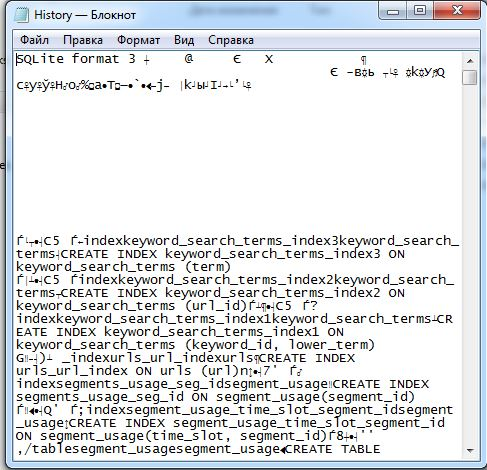
\includegraphics[width=0.6\linewidth]{history}}
\caption{Файл History}
\label{history:history}
\end{figure}

% рисунок - Структура файла Bookmarks
Структура файла Bookmarks приведена на рисунке~\ref{bookmarks:bookmarks}, файла Prefences --- на рисунке~\ref{preferences:preferences}.

\begin{figure}[h!]
\center{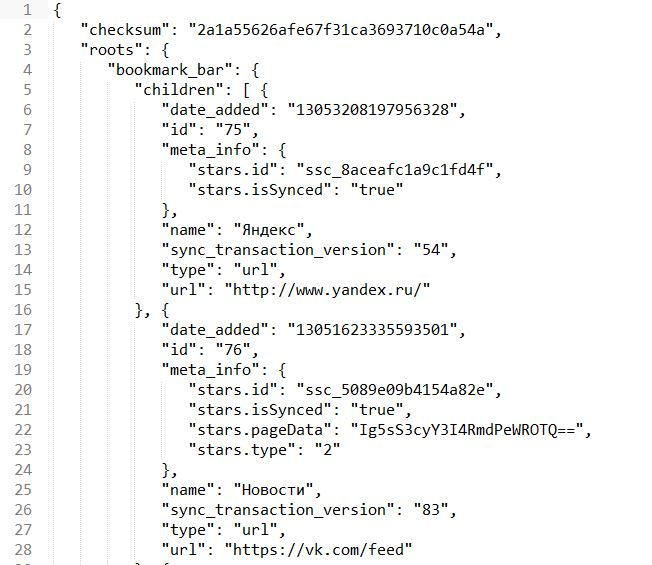
\includegraphics[width=0.6\linewidth]{bookmarks}}
\caption{Структура файла Bookmarks}
\label{bookmarks:bookmarks}
\end{figure}

% рисунок - Структура файла Prefences

\begin{figure}[h!]
\center{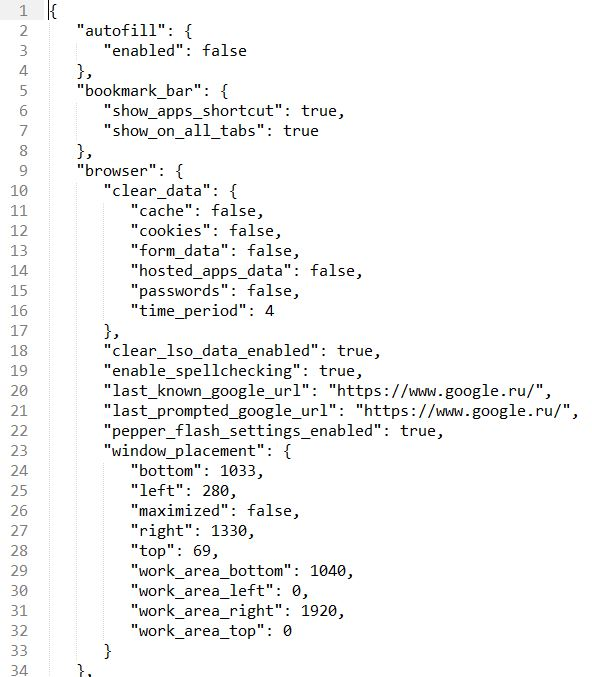
\includegraphics[width=0.6\linewidth]{preferences}}
\caption{Структура файла Preferences}
\label{preferences:preferences}
\end{figure}

Необходимо рассмотреть структуру файла History .sqlite. БД содержит 9 таблиц:
\begin{enumerate}
  \item downloads
  \item downloads\_url\_chains
  \item keyword\_search\_terms
  \item meta
  \item segment\_usage
  \item segments
  \item urls
  \item visit\_source
  \item visits 
\end{enumerate}


Таблицы которые были рассмотрены на данный момент: 
\begin{enumerate}
  \item downloads
  \item downloads\_url\_chains
  \item keyword\_search\_terms
  \item urls
\end{enumerate} 


Таблица downloads содержит информацию о загруженных файлах (путь, время начала загрузки, размер файла, тип файла), но не содержит адрес, откуда был загружен данный файл. Необходимый адрес находится в таблице downloads\_url\_ chains, которая  связана с таблицей downloads по полю id. 
SQL запрос для выборки информации о истории загруженных файлов: SELECT downloads.target\_path, downloads.referrer, downloads.start\_time, downloads.received\_bytes,
downloads\_ url\_ chains.url FROM downloads, downloads\_ url\_ chains WHERE downloads.id=downloads\_ url\_ chains.id.


Пример таблицы downloads можно увидеть на рисунке~\ref{down:down}.

\begin{figure}[ht]
\center{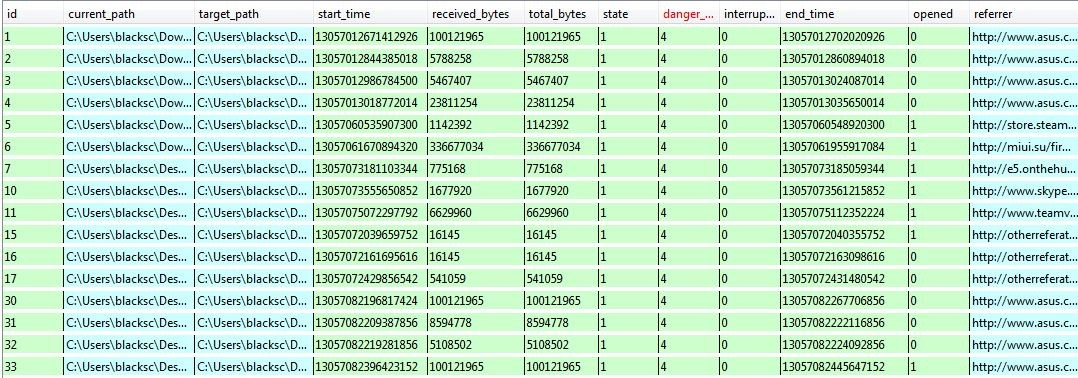
\includegraphics[width=0.9\linewidth]{down}}
\caption{Таблица downloads}
\label{down:down}
\end{figure}

Таблица  keyword\_search\_terms содержит информацию о поисковых запросах (рис.~\ref{key:key}). SQL запрос: SELECT DISTINCT term FROM keyword\_search\_terms.

\begin{figure}[ht]
\center{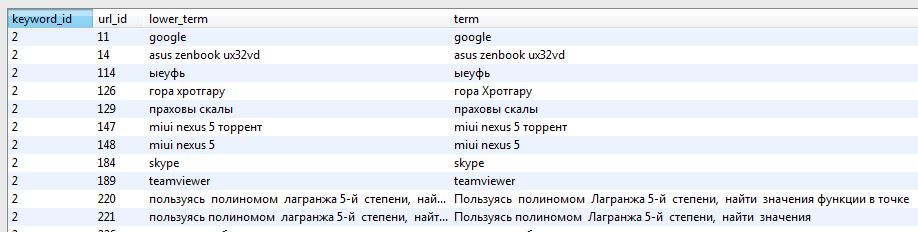
\includegraphics[width=0.9\linewidth]{key}}
\caption{Таблица keyword\_search\_terms}
\label{key:key}
\end{figure}

Таблица  urls содержит информацию о посещенных ресурсах (адрес, заголовок, время последнего посещения). SQL запрос: SELECT url,title,last\_visit\_time FROM urls. Данная таблица приведена на рисунке~\ref{urls:urls}. На рисунке~\ref{chains:chains}, приведена таблица downloads\_url\_chains.

\begin{figure}[h!]
\center{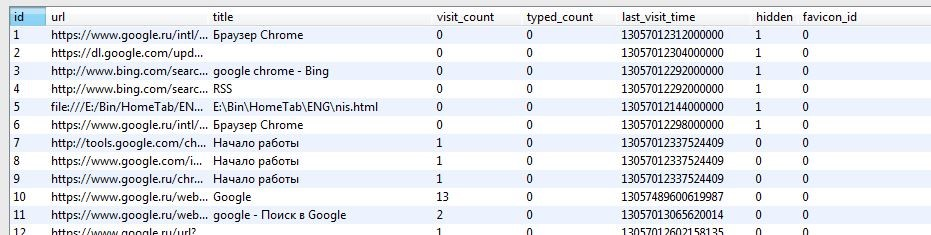
\includegraphics[width=0.9\linewidth]{urls}}
\caption{Таблица urls}
\label{urls:urls}
\end{figure}

\begin{figure}[h!]
\center{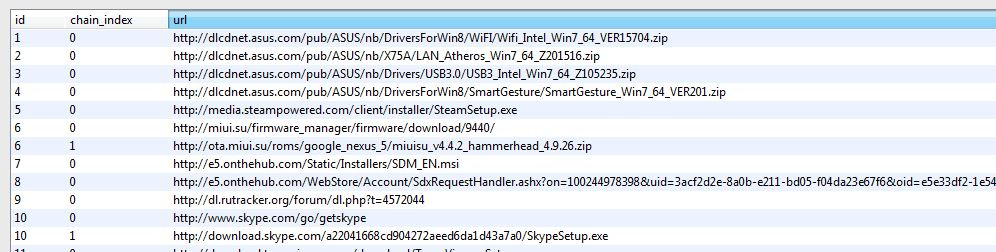
\includegraphics[width=0.9\linewidth]{chains}}
\caption{Таблица downloads\_url\_chains}
\label{chains:chains}
\end{figure}

Как можно увидеть из рисунка~\ref{bookmarks:bookmarks}, структура файла Bookmarks такова: имеется заголовок <<roots>> --- корень, после которого следует подзаголовок <<bookmark\_bar>>, в  теле которого находятся все закладки, расположенные на панели закладок. Тело разбито на блоки, в которых находится такая информация, как дата добавления, адрес ресурса, заголовок страницы. Также присутствует подзаголовок <<other>>, в теле которого находятся все остальные закладки.



В файле Preferences хранится вся возможная информация о настройке браузера. Необходимая информация (версия,  директория загрузки и сохранённый логин) была найдена простым поиском слов (chrome\_version, default\_directory\_download, username) в файле.

\subsubsection{Алгоритм работы модуля}


Блок-схема алгоритма парсинга файла Bookmarks представлена на рисунке~\ref{bookmarks_parsing:bookmarks_parsing}.
% блок-схема парсинга файла Bookmarks
\begin{figure}[h]
\center{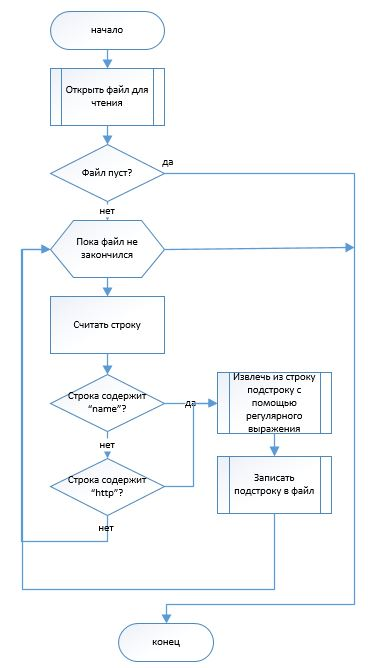
\includegraphics[width=0.6\linewidth]{bookmarks_parsing}}
\caption{Блок-схема алгоритма парсинга файла Bookmarks}
\label{bookmarks_parsing:bookmarks_parsing}
\end{figure}



Извлечение подстроки из строки осуществляется с помощью регулярного выражения: \textbackslash "(.*)\textbackslash".*\textbackslash"(.*)\textbackslash".
Например есть строка "name": "Яндекс", данное регулярное выражение возвращает 2 подстроки name и Яндекс. Из строки "url": "http://www.yandex.ru/" будет найдено url и http://www.yandex.ru/ .Нам необходимы только подстроки с названием страницы и адресом. 

% блок-схема парсинга файла Preferences
Блок-схема алгоритма парсинга файла Preferences представлена на рисунке~\ref{prefences_parsing:prefences_parsing}.

\begin{figure}[h!]
\center{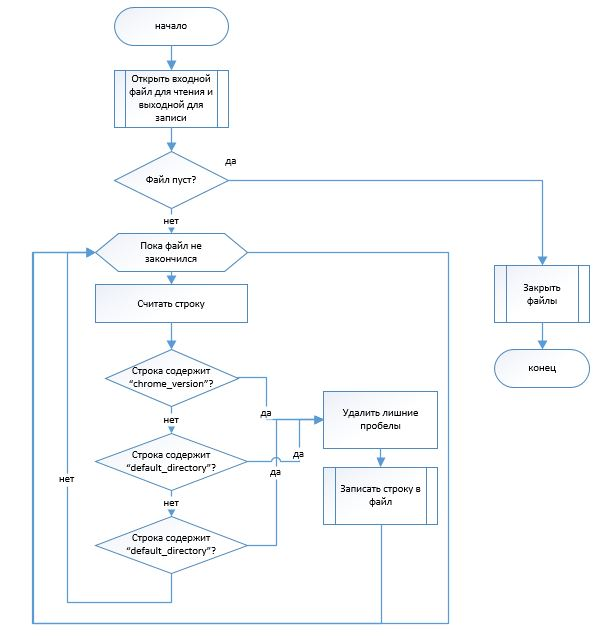
\includegraphics[width=0.9\linewidth]{prefences_parsing}}
\caption{Блок-схема алгоритма парсинга файла Preferences}
\label{prefences_parsing:prefences_parsing}
\end{figure}

% блок-схема алгоритма выборки данных из БД History
Блок-схема алгоритма выборки данных из БД History представлена на рисунке~\ref{history_select:history_select}.

\begin{figure}[h!] 
\center{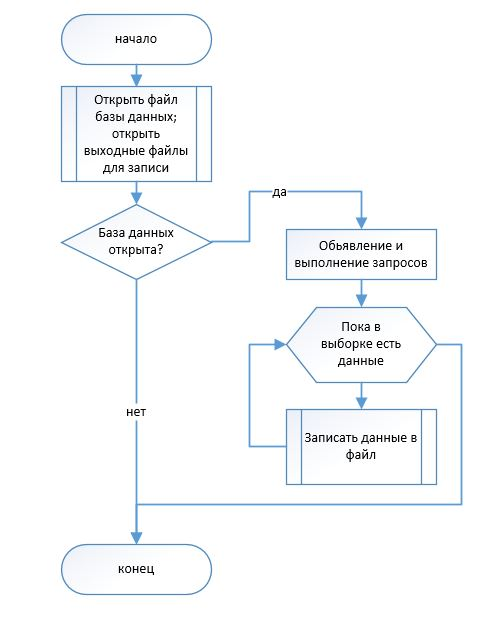
\includegraphics[width=0.6\linewidth]{history_select}}
\caption{Блок-схема алгоритма выборки данных из БД History}
\label{history_select:history_select}
\end{figure}


\subsubsection{Структура логов, записанных в формате XML} 
Документы XML имеют иерархическую структуру и начинаются с пролога, который указывает, что документ написан на XML, а также указывает версию XML. Следующий элемент <add> --- это начальный элемент документа (корень). Далее будут записаны n дочерних элементов <doc> где n --- количество обьектов, в теле которых будет записано нужное нам количество полей для записи информации. В последнюю очередь записывается конечный элемент </add>.

Пример файла bookmarks.XML приведен на рисунке~\ref{bookmarks_xml:bookmarks_xml}.

\begin{figure}[ht]                                            % здесь рисунок bookmarks_xml
\center{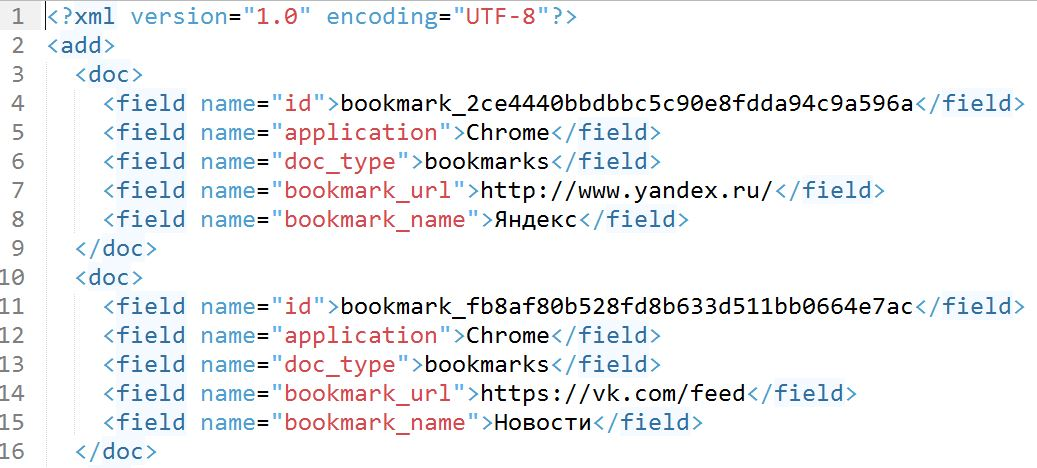
\includegraphics[width=0.6\linewidth]{bookmarks_xml}}
\caption{Файл bookmarks.XML}
\label{bookmarks_xml:bookmarks_xml}
\end{figure}

Значение поля id --- это сгенерированный хэш MD5 от строки bookmark\_ url + <<Chrome>>, application --- наименование приложения, doc\_type --- тип информации (рис.~\ref{bookmarks_xml:bookmarks_xml}).

\begin{figure}[ht]                                          % еще рисунок preferences_xml
\center{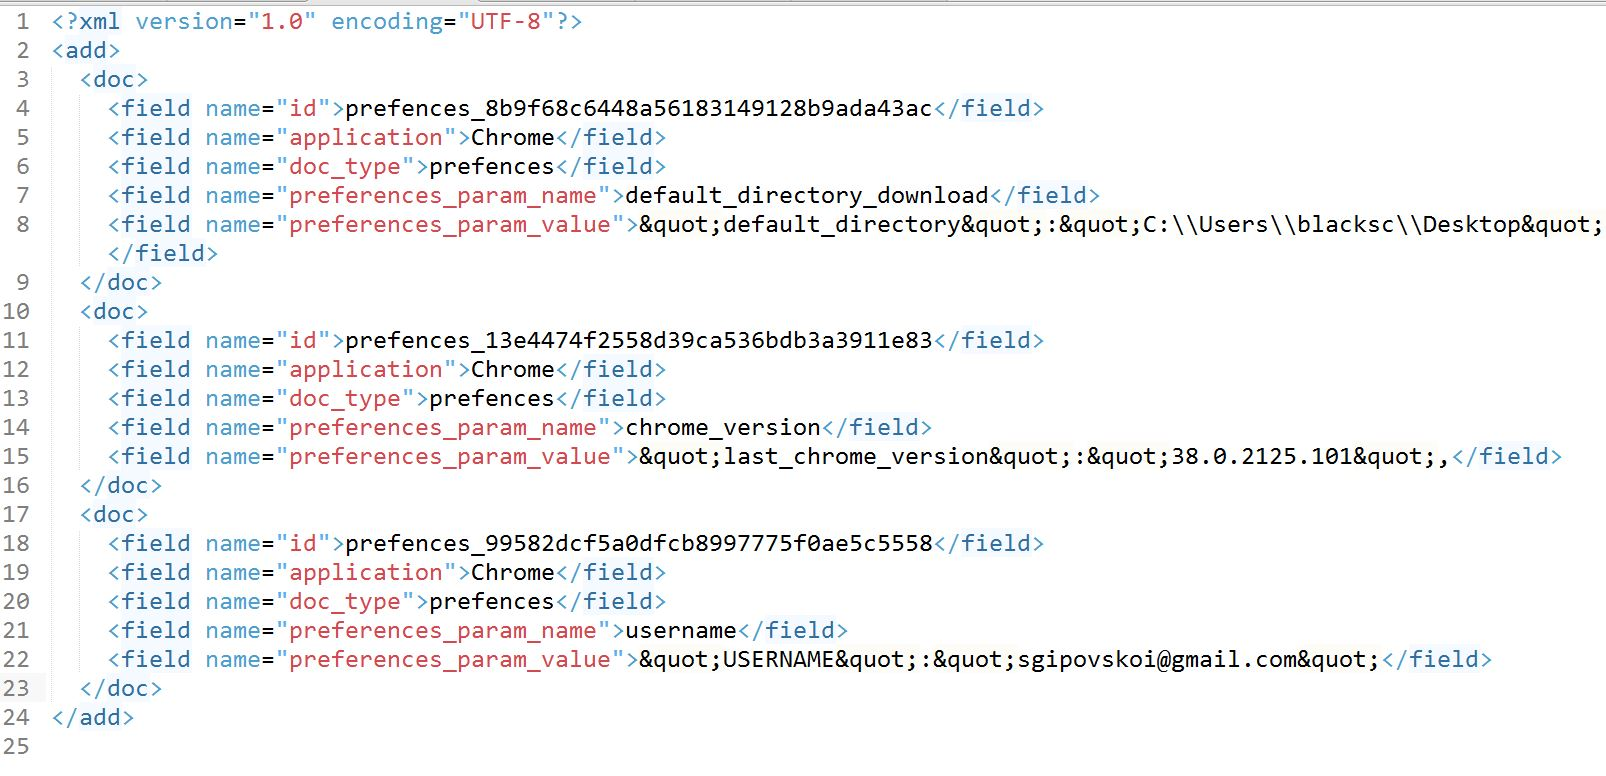
\includegraphics[width=0.8\linewidth]{preferences_xml}}
\caption{Файл preferences.XML}
\label{preferences_xml:preferences_xml}
\end{figure}

Значение поля id --- это сгенерированный хэш MD5 от строки preferences\_ param\_ value + <<Chrome>> (рис.~\ref{preferences_xml:preferences_xml}).

\begin{figure}[ht]                                           % и тут рисунок файл history_xml
\center{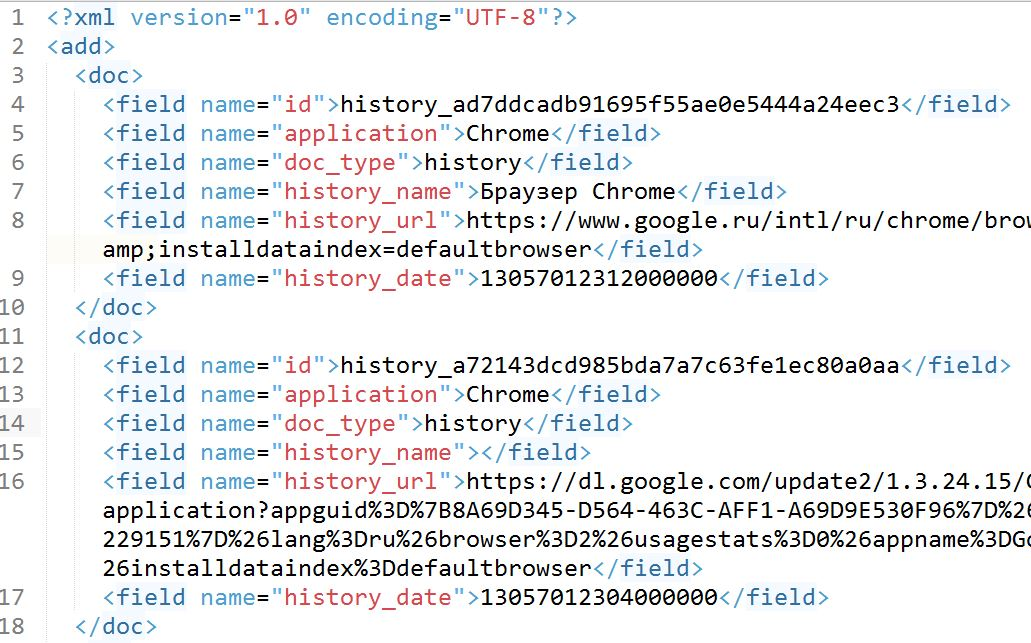
\includegraphics[width=0.6\linewidth]{history_xml}}
\caption{Файл history.XML}
\label{history_xml:history_xml}
\end{figure}

Значение поля id --- это сгенерированный хэш MD5 от строки history\_ name + history\_ url + history\_ date + <<Chrome>> (рис.~\ref{history_xml:history_xml}).

\begin{figure}[ht]                                            % и тут рисунок download_xml
\center{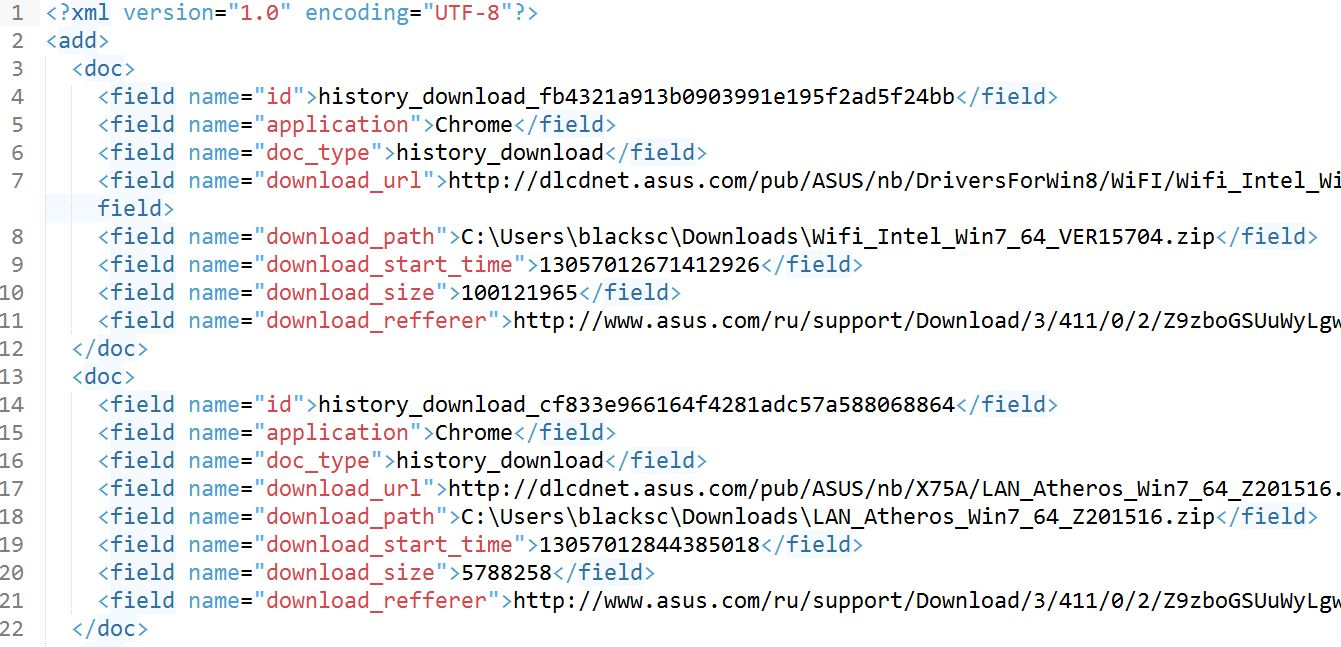
\includegraphics[width=0.8\linewidth]{download_xml}}
\caption{Файл download.XML}
\label{download_xml:download_xml}
\end{figure}

Значение поля id --- это сгенерированный хэш MD5 от строки <<download>> + dowload\_ url + dowload \_ start \_ time + <<Chrome>> (рис.~\ref{download_xml:download_xml}). Значение download\_size записывается в байтах.


Значение поля id --- это сгенерированный хэш MD5 от строки keyword\_ term + <<Chrome>> (рис.~\ref{search_term_xml:search_term_xml}).

\begin{figure}[!pHt]                                          % и тут рисунок search_term_xml
\center{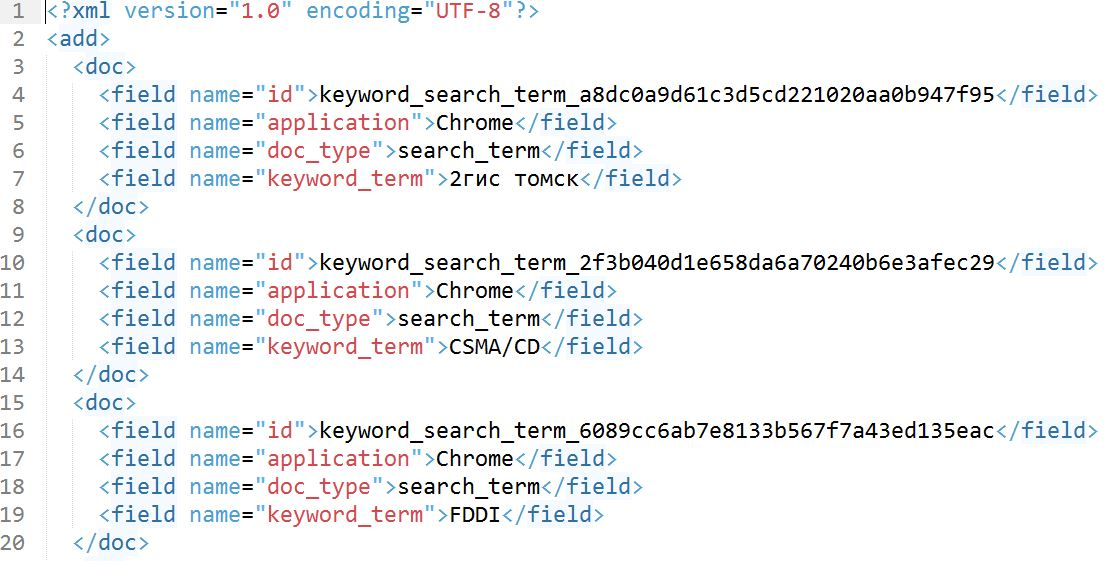
\includegraphics[width=0.9\linewidth]{search_term_xml}}
\caption{Файл search\_term.XML}
\label{search_term_xml:search_term_xml}
\end{figure}

На данный момент реализован импорт истории (посещений, поисковых запросов, загруженных файлов), закладок и 
другой информации (версия приложения, логин аккаунта google) из приложения Google Chrome.

\subsubsection{Задачи на слудующий семестр}
\begin{enumerate}
  \item Добавить модуль к общему комплексу.
  \item Нормализовать формат даты.
  \item Реализовать рекурсивный обход файловой системы для нахождения необходимых файлов.
  \item Поиск другой информации приложения Google Chrome.
\end{enumerate}

\clearpage
